% --------- Introduction ---------
\section{Introduction}
\label{sec:intro}




\subsection{System concepts}
\label{subsec:sysbase}


\begin{frame}
  \frametitle{What is a CPU ?}

  \begin{itemize}
  \item Execute sequences of instruction
  \item Fetched from the memory through caches
  \item Operates on
    \begin{itemize}
    \item Registers
    \item Memory (through caches)
    \end{itemize}
  \item Registers:
    \begin{itemize}
    \item General purposes
    \item PC
    \item Stack pointer (BP/SP)
    \item Various statuses
    \end{itemize}
  \end{itemize}
\end{frame}




\begin{frame}
  \frametitle{CPU Execution pipeline}

  \begin{center}
    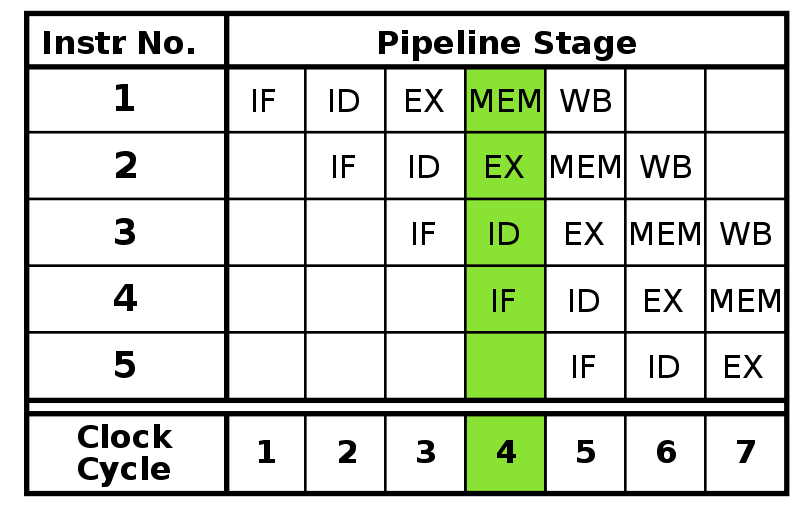
\includegraphics[width=0.8\textwidth,height=0.4\textheight,keepaspectratio]{img/cpu_pipeline.png}
  \end{center}


  \begin{itemize}
  \item IF = Instruction fetch
  \item ID = Instruction decode
  \item EX = Execute
  \item MEM = Memory access
  \item WB = Write back
  \end{itemize}
\end{frame}



\begin{frame}
  \frametitle{Memory}

  \begin{itemize}
  \item Arrays of bytes for the CPU to work on
  \item Organized in Hierarchy:
    \begin{itemize}
    \item register > caches > main memory > disk / networks
    \end{itemize}
  \item A few numbers\footnote{https://gist.github.com/jboner/2841832}:
    \begin{itemize}
    \item Register: no latency (0-2 cycles)
    \item Caches:
      \begin{itemize}
      \item L1: ~ 0.5 ns
      \item L2: ~ 7 ns
      \item L3: ~ 15 ns
      \end{itemize}
    \item Memory: ~ 100 ns
    \item SSD: ~ 150 us
    \item Disk read: ~ 1ms
    \item US ping: ~ 150 ms
    \end{itemize}
  \end{itemize}
\end{frame}

\begin{frame}
  \frametitle{}

  \begin{center}
    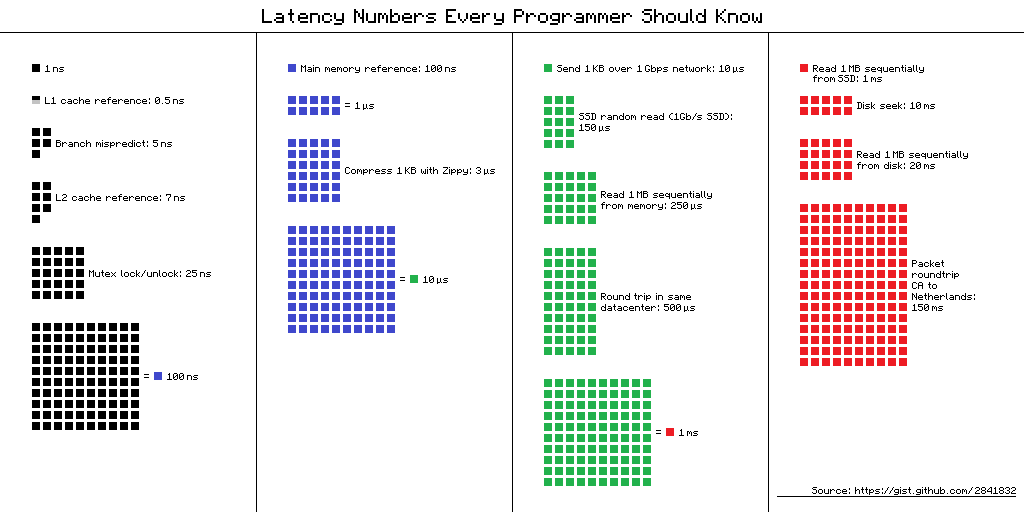
\includegraphics[width=1\textwidth,height=1\textheight,keepaspectratio]{img/latency.png}
  \end{center}

\end{frame}

\begin{frame}
  \frametitle{Non-Uniform Memory Access}

  \begin{itemize}
  \item NUMA for short
  \item Memory is split in nodes
  \item Each core has direct access to only one node
  \item Access to other nodes is shared (slower)
  \item Different NUMA layouts
    \begin{itemize}
    \item 1:1
    \item 1:n
    \end{itemize}
  \end{itemize}

  \begin{center}
    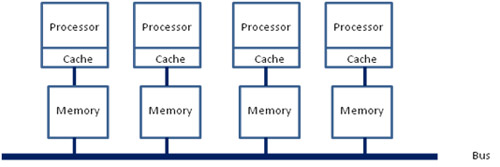
\includegraphics[width=0.8\textwidth,height=0.5\textheight,keepaspectratio]{img/numa.jpg}
  \end{center}
\end{frame}


\begin{frame}
  \frametitle{Virtual memory}

  \begin{itemize}
  \item Real/Direct mode
    \begin{itemize}
    \item Programs access memory directly
    \item 0x00 $\rightarrow$ first byte of memory
    \item Unsafe!
    \end{itemize}
  \item Virtual/Protected mode
    \begin{itemize}
    \item Programs addresses are mapped to different addresses
    \item 0x00 $\rightarrow$ unknown
    \item Safe !
    \item Kernel maintains mapping (page directory)
    \item MMU / TLB
    \end{itemize}
  \end{itemize}
\end{frame}


\begin{frame}
  \frametitle{Context switching}

  \begin{itemize}
  \item Stopping the execution of a program to run another
  \item What is a context ?
    \begin{itemize}
    \item Registers (pc, stack, ...)
    \item Memory mappings (pagedir, TLB)
    \end{itemize}
  \item Save the current context, load another
  \item Costly !
  \end{itemize}
\end{frame}


\begin{frame}
  \frametitle{Multitasking}

  \begin{itemize}
  \item Multiple program
  \item in their ``own memory''
  \item running ``at the same time''
  \item but actually sharing Memory and CPU Time
  \item Understanding the kernel is \textbf{vital}
  \end{itemize}
\end{frame}




\subsection{Parallel computing}

\begin{frame}
  \frametitle{What is parallel computing ?}

  \begin{quotation}
    Parallel computing is a type of computation in which many calculations are carried out simultaneously, operating on the principle that large problems can often be divided into smaller ones, which are then solved at the same time.
    There are several different forms of parallel computing: bit-level, instruction-level, data, and task parallelism.
    Parallelism has been employed for many years [...] but interest in it has grown lately due to the physical constraints preventing frequency scaling.
  \end{quotation}
  \emph{Wikipedia}
\end{frame}

\begin{frame}
  \frametitle{Instruction-level parallelism}
  \begin{itemize}
  \item Instruction pipelining
  \item Branch prediction
    \begin{itemize}
    \item Predict \emph{if-then-else} to prefetch code
    \end{itemize}
  \item Hyper-threading
    \begin{itemize}
    \item \emph{Logical} core
    \item Fill the bubbles in the instruction pipeline
    \end{itemize}
  \item ...
  \end{itemize}
\end{frame}

\begin{frame}
  \frametitle{Task/Data-level parallelism}
  \begin{itemize}
  \item Task Level
    \begin{itemize}
    \item Do X and Y in parallel
    \item Pipeline pattern
    \end{itemize}
  \item Data-level
    \begin{itemize}
    \item Split X and split the parts in parallel
    \item SIMD
    \item Producer/consumer pattern
    \end{itemize}
  \item Some overlap between the two
  \item More on this topic later
  \end{itemize}
\end{frame}


\begin{frame}
  \frametitle{Why parallelism matters ?}
  \begin{itemize}
  \item Frequency scaling vs multi-core
  \item Operating systems are multitask
  \item Latency control
  \item Important even for non-parallel programs
  \end{itemize}
\end{frame}


\begin{frame}
  \frametitle{Some history}

  \begin{itemize}
  \item Context switching for batches \emph{(Leo III, UK, 1961)}
  \item Cooperative multitasking Time-sharing \emph{(CTSS, MIT, 1961)}
    \begin{itemize}
    \item IBM, MacOS, Win 3.1/9.x
    \end{itemize}
  \item Preemptive multitasking \emph{(Multics, Cambridge, 1964)}
    \begin{itemize}
    \item Multics, very influential OS.
    \item Linux, OSX, Win NT+
    \item Most OSes today
    \end{itemize}
  \item Virtual memory \emph{(Atlas/Burroughs, 1961/1962)}
  \item Threads \emph{(OS/360, IBM, 1967)}
  \end{itemize}
\end{frame}





\subsection{The Unix/Linux model}
\label{subsec:linuxmodel}


\begin{frame}
  \frametitle{POSIX}

  \begin{itemize}
  \item \emph{Many} UNIXes (Linux, BSDs, HP-UX, AIX, Solaris, ...)
  \item Common features and semantic
    \begin{itemize}
    \item Virtual Memory
    \item Preemptive multitasking
    \item File system
    \item Shell
    \item Written in C
    \end{itemize}
  \item Standardization effort
    \begin{itemize}
    \item Portable Operating System Interface (IEEE, 1988-2008)
    \item Single Unix Specification (Austin Group, 1997-2008)
    \end{itemize}
  \end{itemize}
\end{frame}


\begin{frame}
  \frametitle{Processes}

  \begin{itemize}
  \item A running program
  \item Container of resources
    \begin{itemize}
    \item Memory
    \item File descriptors
    \item Execution path
    \item ...
    \end{itemize}
  \item Coordinated by the kernel
    \begin{itemize}
    \item Scheduler
    \item Communication (pipes, shared memory)
    \item Synchronization (locks, semaphores)
    \end{itemize}
  \item Unix parallelism is process based
  \end{itemize}
\end{frame}


\begin{frame}
  \frametitle{fork()}

  \begin{itemize}
  \item The Unix process creation model:
    \begin{itemize}
    \item Process duplication: \emph{fork()}
    \item Process image replacement: \emph{exec()} family
    \item Take care of lifecycle management !
    \end{itemize}
  \item Creating processes is \emph{cheap}
    \begin{itemize}
    \item unlike Windows
    \item Many optimizations (COW, ...)
    \end{itemize}
  \end{itemize}
\end{frame}


\begin{frame}[fragile]
  \frametitle{fork() example}

  \begin{minted}{c}
    pid_t pid = fork();
    if (pid) {
      // Parent (original process)
      int status;
      wait(&status); // Ask if you don't know
    } else {
      // Child (new process)
      char *newenviron[] = { NULL };
      char *newargv[] = { NULL };

      // Replace the current process by "/bin/ls"
      execve("bin/ls", newargv, newenviron);
    }
  \end{minted}
\end{frame}



\begin{frame}
  \frametitle{Threads}

  \begin{itemize}
  \item a.k.a \emph{Lightweight processes}
  \item \emph{Relatively recent} in UNIX history
  \item Task with shared resources
    \begin{itemize}
    \item Memory space
    \item File descriptors
    \item ...
    \end{itemize}
  \item Multiple execution path within a process
    \begin{itemize}
    \item 1 process: 1-n threads
    \end{itemize}
  \item Separate stack and registers
  \end{itemize}
\end{frame}


\begin{frame}
  \frametitle{clone()}

  \begin{itemize}
  \item In Linux, \emph{fork()} wraps \emph{clone()}
  \item Duplicate tasks
    \begin{itemize}
    \item Task: kernel name for execution context + resources
    \item Something \emph{schedulable}
    \end{itemize}
  \item Choose what you share or copy/reset:
    \begin{itemize}
    \item Memory
    \item File descriptors
    \item Network namespace, ...
    \end{itemize}
  \item Share everything: You're a thread !
    \begin{itemize}
    \item \emph{and a hippie :)}
    \end{itemize}
  \end{itemize}
\end{frame}
